\cfoot{Hannah Siegel}
\textit{RoboNav} is designed to enrich the positioning and the navigation of a mobile robot with information from an overhead camera and therefore improving the navigation. The final version of the project showed, that this theoretical idea can be accomplished, but maybe not as easy and well-performing as it was expected. \\ \\
The project should work real-time and show a combination of external tracking in terms of positioning and a map-based external navigation possibility to perform ideal movements. \\
The overall system works fine. The path-planning and the path-driving functionality in particular work just as expected. With well-placed obstacles the paths are driven without collisions. Sometimes the path can not be calculated since no possible way was found, but this is not a bug in the path-planning software, it is only an impossible use-case which is simply ignored by the system. The software has the limitation that before starting the path-driver should be started only when having cleaned the  \texttt{RoboNavPath.txt} file before, otherwise the old path will be driven immediately. Furthermore, the robot must always be started facing in a certain direction, as showed in Figure \ref{fig:mirrorx} , in order for the coordinate systems to match.\\ %TODO recheck
The image processing works very accurate. 
It recognizes even bright coloured objects on white ground, but for good results it's better if the obstacles have a easy distinguish color.
\\
The position comparison on the other hand did not deliver the desired results: even trough the position-information from the overhead-camera can be used from time to time in order to gain accuracy, it can not be used in near real time. The reason is mainly the delay of the image-transmission of the streaming-app and the intensive calculations afterwards. \\ This means, that a functioning position comparison should only be carried out when the robot is resting on the same position for at least two seconds but the average case is still faster than half a second. The fact that a comparison is even available, should theoretically improve any navigation already. The outcome of the position comparison can be seen in Figure \ref{fig:bla}. Since the internal odometry of the \textit{Robotino} is of a high quality, the aberrations were hardly measurable after smaller distances. This made it very hard to compare the improvements with and without \textit{RoboNav} on the small testing area the project had available.
\begin{figure}[htb!]
	\begin{minipage}{.3\textwidth}
		\centering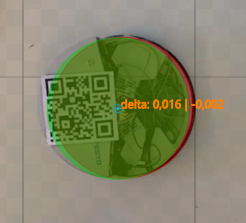
\includegraphics[width=0.8\textwidth]{images/abberation1small}
	\end{minipage}
	\begin{minipage}{.3\textwidth}
		\centering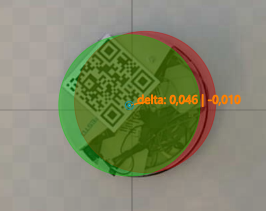
\includegraphics[width=0.9\textwidth]{images/abberation2small}
	\end{minipage}
	\begin{minipage}{.3\textwidth}
		\centering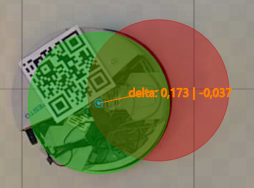
\includegraphics[width=0.9\textwidth]{images/abberation3small}
	\end{minipage}
	\caption[Bla (self-made)]{Aberration at start, after 5 minutes and after 25 minutes}
	\label{fig:bla}
\end{figure}
\FloatBarrier

\textbf{Lessons Learned}\\
The overall idea of the project is fine and the implementation was good enough to ensure an improvement.
For sure, the performance and the speed of processing information could be faster. \textit{Robonav} used Java and therefore ran into some performance and also some parsing problems between the wrapped Java classes and the native C++ library. Maybe using C++ could show some improvements in terms of performance and compatibility issues. Furthermore, even trough the idea of dividing the system into three independent components - \textit{RoboNav Control, RoboNav Overview} and \textit{RoboNav Sight} - is providing a lot of flexibility, it lead to much communication between the components. \\
When working with different systems, such as robots and cameras, the issue of adjusting and scaling their respective coordinates systems should have been considered earlier in the project, since this posed some problems in the final stage of integrating the components, that could not finally be resolved. 
\\\\
%\subsubsection{Ok Conclusio}
%\textbf{Final Outcome changes:} \\
%The overall system works fine. The path-planning and the path-driving functionality in particular work well enough to ensure a stable testing environment but may sometimes fail to execute perfectly. With well-placed obstacles the paths are mostly driven without major collisions. Sometimes the path can not be calculated since no possible way was found, but this is not a bug in the path-planning software, it is only an impossible use-case. The path-driver should be started only when having cleaned the  \texttt{RoboNavPath.txt} file before, otherwise the old path will be driven immediately. Furthermore, the robot must always be started facing XXXX, in order for the coordinate systems to match.\\ 
%\subsubsection{Bad Conclusio}
%\textbf{Final Outcome changes:} \\
%The project should work real-time and show a combination of external tracking in terms of positioning and a map-based external navigation possibility to perform ideal movements. \\
%The path-planning and the path-driving functionality in particular did not work as expected, due to compatibility issues between the coordinate systems of the entities. %With well-placed obstacles the paths are mostly driven without major collisions. Sometimes the path can not be calculated since no possible way was found, but this is not a bug in the path-planning software, it is only an impossible use-case.
%The path-driver should be started only when having cleaned the  \texttt{RoboNavPath.txt} file before, otherwise the old path will be driven immediately. Furthermore, the robot must always be started facing XXXX, in order for the coordinate systems to match.\\ \\
%\textbf{other  changes:} \\
% The fact that a comparison is even available, should theoretically improve any navigation already. Since the internal odometry of the \textit{Robotino} is very high-class, the aberrations of it were hardly measurable after smaller distances. Furthermore, the fact that the navigation component of the system failed to work absolutely fine without eventual bugs, it is not possible to test it over an longer timespan. This made it very hard to compare the improvements with and without \textit{RoboNav}.
\textbf{Outlook}\\
Since the demand for robots is generally growing, their navigation-possibilities will improve as well. Maybe vision based systems are a technology which will get used even more in the future. \\
The \textit{RoboNav} project could be expanded by the following ideas:
\begin{enumerate}
\item \textit{RoboNav} was tested with only one robot, but it was designed for more than that. The usage of more than one robot generates issues such as crossing pathways, priorities or different hardware and software requirements. \\ Whenever using more than one robot, topics like task sharing or intelligent systems may be explored. 
\item  There was only one overhead camera in use. By combining more images, either from a wider range or from different perspectives, more information might have been provided.
\item By programming the \textit{RoboNav Control} in order to gain "\textit{artificial intelligence}", it could take over tasks such as classifing and checking obstacles and using fuzzy sets for handling these obstacles. This would improve the overall navigation due to cutting out eventual errors from the image processing.   
\item \textit{RoboNav} could be integrated into other programming languages, therefore enabling an easier handling of the functions. Blocks for the \textit{RobotinoView} program could help an user to evade the usage of files.
\item The overview camera might be exchanged for a high-resolution industrial camera, therefore delivering faster and better pictures than the android smartphone does. The transmission of the pictures could be implemented in a faster way as well, for example by using two connections - one for the \textit{RoboNav Control} and one for the \textit{RoboNav Overview}. 
\end{enumerate} 

